\documentclass[review,onefignum,onetabnum]{siamart190516}
%\usepackage{natbib}
%\usepackage[sort]{cite}
\pdfoutput=1
%\usepackage[colorlinks=true,urlcolor=blue,citecolor=blue,linkcolor=blue]{hyperref}
\usepackage[english]{babel}
\usepackage[utf8]{inputenc}
\usepackage[T1]{fontenc}
\usepackage{amssymb}
\usepackage{tabularx}
\usepackage{quoting}
\usepackage{upquote}
\usepackage{subcaption}
\usepackage{multicol}
\usepackage{cancel}
\usepackage[framemethod=TikZ]{mdframed}
\usetikzlibrary{shapes}
\usetikzlibrary{snakes}
\usepackage{wrapfig}
%\usepackage{caption}
%\usepackage[plain]{algorithmic}
\usepackage[linesnumbered, ruled, vlined, algo2e]{algorithm2e}
\usepackage{algpseudocode}
\usepackage{rotating}
%\usepackage{cite}
\usepackage{booktabs}
%\usepackage{unicode-math}
%\usepackage{algorithm}% http://ctan.org/pkg/algorithm
%\usepackage{algpseudocode}% http://ctan.org/pkg/algpseudocode
\usepackage{xcolor}% http://ctan.org/pkg/xcolor
\makeatletter
\newsavebox{\@brx}
\newcommand{\llangle}[1][]{\savebox{\@brx}{\(\m@th{#1\langle}\)}%
  \mathopen{\copy\@brx\kern-0.5\wd\@brx\usebox{\@brx}}}
\newcommand{\rrangle}[1][]{\savebox{\@brx}{\(\m@th{#1\rangle}\)}%
  \mathclose{\copy\@brx\kern-0.5\wd\@brx\usebox{\@brx}}}
\makeatother
\usepackage{bbm}
\usepackage{jlcode}
\usepackage{graphicx}
\usepackage{amsmath,color}
\usepackage{mathrsfs}
\usepackage{float}
\usepackage[normalem]{ulem}
\usepackage{makecell}
\usepackage{indentfirst}
\usepackage{txfonts}
\usepackage[epsilon, tsrm, altpo]{backnaur}

\makeatletter
\def\parsept#1#2#3{%
    \def\nospace##1{\zap@space##1 \@empty}%
    \def\rawparsept(##1,##2){%
        \edef#1{\nospace{##1}}%
        \edef#2{\nospace{##2}}%
    }%
    \expandafter\rawparsept#3%
}
\makeatother
\DeclareMathAlphabet{\mymathbb}{U}{BOONDOX-ds}{m}{n}
\newcommand{\listingcaption}[1]%
{%
\refstepcounter{lstlisting}\hfill%
Listing \thelstlisting: #1\hfill%\hfill%
}%
\newcolumntype{b}{X}
\newcolumntype{s}{>{\hsize=.7\hsize}X}
\usepackage{listings}
\lstset{
    language=Julia,
    basicstyle=\ttfamily\scriptsize,
    numberstyle=\scriptsize,
    % numbers=left,
    backgroundcolor=\color{gray!7},
    %backgroundcolor=\color{white},
    %frame=single,
    xleftmargin=2em,
    tabsize=2,
    rulecolor=\color{black!15},
    %title=\lstname,
    escapeinside={(*}{*)},
    breaklines=true,
    %breakatwhitespace=true,
    %framextopmargin=2pt,
    %framexbottommargin=2pt,
    frame=bt,
    extendedchars=true,
    inputencoding=utf8,
    columns=fullflexible,
    %escapeinside={(*@}{@*)},
}

\tolerance=1
\emergencystretch=\maxdimen
\hyphenpenalty=1000
\hbadness=1000

\makeatletter

%%%%%%%%%%%%%%%%%%%%%%%%%%%%%% User specified LaTeX commands.

%Journal reference.  Comma sets off: name, vol, page, year
\def\journal #1, #2, #3, 1#4#5#6{{\sl #1~}{\bf #2}, #3 (1#4#5#6) }
\def\pr{\journal Phys. Rev., }
\def\prb{\journal Phys. Rev. B, }
\def\prl{\journal Phys. Rev. Lett., }
\def\pl{\journal Phys. Lett., }
%\def\np{\journal Nucl. Phys., }


%%%%%%%%%%%%%%%%%%%%%%%%%%%%%%%%%%%%%%%%%%%%%%%%%%%%%%%%%%%%%%%%%%%%%%%%%%%%%%%%%%%%%%%%%%%%%%%%%%%%%%%%%%%%%%%%%%%%%%%%%%%%%%%%%%%%%%%%%%%%%%%%%%%%%%%%%%%%%%%%%%%%%%%%%%%%%%%%%%%%%%%%%%%%%%%%%%%%%%%%%%%%%%%%%%%%%%%%%%%%%%%%%%%%%%%%%%%%%%%%%%%%%%%%%%%%


%\usepackage{CJK}
%\usepackage[colorlinks, citecolor=blue]{hyperref}
\DeclareMathOperator*{\argmax}{arg\,max}

%%%%%% Shortcut related
\newcommand{\<}{\langle}
\renewcommand{\>}{\rangle}
\newcommand{\out}{{\vx^L}}
\newcommand{\inp}{{\vx^0}}
\newcommand{\cquad}{{{ }_{\quad}}}
\newcommand{\pluseq}{\mathrel{+}=}
\newcommand{\minuseq}{\mathrel{-}=}
\newcommand{\vx}{{\mathbf{x}}}
\newcommand{\vg}{{\mathbf{g}}}
\newcommand{\vp}{{\mathbf{p}}}
\newcommand{\vy}{{\mathbf{y}}}
\newcommand{\Var}{{\mathrm{Var}}}
\newcommand{\Mean}{{\mathrm{E}}}
\newcommand{\vvalue}{{\texttt{value}}}
\newcommand{\grad}{{\texttt{grad}}}
\newcommand{\parameter}{{\texttt{parameter}}}
%%%%%% Convention related
\newcommand{\SWAP}{{\rm SWAP}}
\newcommand{\CNOT}{{\rm CNOT}}
\newcommand{\bigO}{{\mathcal{O}}}
\newcommand{\X}{{\rm X}}
\renewcommand{\H}{{\rm H}}
\newcommand{\Rx}{{\rm Rx}}
\renewcommand{\v}[1]{{\bf #1}}
\newcommand{\dataset}{{\mathcal{D}}}
\newcommand{\wfunc}{{\psi}}
\newcommand{\SU}{{\rm SU}}
\newcommand{\UU}{{\rm U}}
\newcommand{\thetav}{{\boldsymbol{\theta}}}
\newcommand{\gammav}{{\boldsymbol{\gamma}}}
\newcommand{\thetai}{{\theta^\alpha_l}}
\newcommand{\Expect}{{\mathbb{E}}}
\newcommand{\Tr}{{\rm Tr}}
\newcommand{\etc}{{\it etc~}}
\newcommand{\etal}{{\it etal~}}
\newcommand{\xset}{\mathbf{X}}
\newcommand{\fl}{\texttt{fl}}
\newcommand{\pdata}{\mathbf{\pi}}
\newcommand{\q}{\mathbf{q}}
\newcommand{\epdata}{\mathbf{\hat{\pi}}}
\newcommand{\gammaset}{\boldsymbol{\Gamma}}
\newcommand{\ei}{{\mathbf{e}_l^\alpha}}
\newcommand{\vtheta}{{\boldsymbol{\theta}}}
\newcommand{\sigmag}{{\nu}}
\newcommand{\sigmai}[2]{{\sigma^{#2}_{#1}}}
\newcommand{\qi}[1]{{q^{\alpha_{#1}}_{#1}}}
\newcommand{\BAS}{Bars-and-Stripes}
\newcommand{\circled}[1]{\raisebox{.5pt}{\textcircled{\raisebox{-.9pt} {#1}}}}
\newcommand{\qexpect}[1]{{\left\langle #1\right\rangle}}
\newcommand{\expect}[2]{{\mathop{\mathbb{E}}\limits_{\substack{#2}}\left[#1\right]}}
\newcommand{\var}[2]{{\mathop{\mathrm{Var}}\limits_{\substack{#2}}\left(#1\right)}}
\newcommand{\pshift}[1]{{p_{\thetav+#1}}}
\newcommand{\upcite}[1]{\textsuperscript{\cite{#1}}}
\newcommand{\Eq}[1]{Eq.~(\ref{#1})}
\newcommand{\Fig}[1]{Fig.~\ref{#1}}
\newcommand{\Lst}[1]{Listing.~\ref{#1}}
\newcommand{\Tbl}[1]{Table~\ref{#1}}
\newcommand{\Sec}[1]{Sec.~\ref{#1}}
\newcommand{\App}[1]{Appendix~\ref{#1}}
\newcommand{\bra}[1]{\mbox{$\left\langle #1 \right|$}}
\newcommand{\ket}[1]{\mbox{$\left| #1 \right\rangle$}}
\newcommand{\braket}[2]{\mbox{$\left\langle #1 | #2 \right\rangle$}}
\newcommand{\tr}[1]{\mathrm{tr}\mbox{$\left[ #1\right]$}}

\newcommand{\ra}[1]{\renewcommand{\arraystretch}{#1}}

%%%%%% Comment related
\newcommand{\red}[1]{[{\bf  \color{red}{ST: #1}}]}
\newcommand{\xred}[1]{[{\bf  \color{red}{\sout{ST: #1}}}]}
\newcommand{\green}[1]{[{\bf  \color{green}{XG: #1}}]}
\newcommand{\xgreen}[1]{[{\bf  \color{green}{\sout{XG: #1}}}]}
\newcommand{\blue}[1]{[{\bf  \color{blue}{JG: #1}}]}
\newcommand{\xblue}[1]{[{\bf  \color{blue}{\sout{JG: #1}}}]}
\newcommand{\material}[1]{\iffalse[{\bf  \color{cyan}{Material: #1}}]\fi}

\newcounter{example}
\newenvironment{example}[1][]{\refstepcounter{example}\par\medskip
   \noindent \textbf{Example~\theexample. #1} \rmfamily}{\medskip}

%\newtheorem{theorem}{\textit{Theorem}}
%\newtheorem{corollary}{\textit Branching Rule}
%\theoremstyle{definition}\newtheorem{definition}{\textit{Definition}}
%\newtheorem{defin}[thm]{Definition}

\makeatother

%\externaldocument{ex_supplement}

\title{Solving the independent set problem by generic programming tensor networks
\thanks{\funding{...}}
}

\author{XXX\thanks{XXX 
  (\email{email}, \url{website}).}
\and YYY\thanks{yyyyy 
  (\email{yyyy}, \email{email}).}
}

\begin{document}

\maketitle

\begin{abstract}
	This paper is about solving the independent set problem by eincoding this problem to a tensor network. 
    We show how to obtain the maximum independent set size, the independence polynomial and optimal configurations of a graph by engineering the tensor element algebra.
    We also show how to analyse the local properties of a graph by contracting an open tensor network.
\end{abstract}

% REQUIRED
\begin{keywords}
  maximum independent set, tensor network
\end{keywords}

% REQUIRED
% 14N07  	Secant varieties, tensor rank, varieties of sums of powers
\begin{AMS}
  05C31, 14N07
\end{AMS}

\section{Introduction}
\blue{efficient counting maximal independent sets~\cite{Manne2013}, overlap gap property~\cite{Gamarnik2013, Gamarnik2019}, independence polynomial at -1~\cite{Bousquet2008,Levit2009}}
In this work, we introduce a tensor based framework to study the famous graph problem of finding independent sets.
Given an undirected graph $G = (V,E)$, an independent set $I \subseteq V$ is a set that for any $u,v \in I$, there is no edge connecting $u$ and $v$ in $G$.
The problem of finding the maximum independent set (MIS) size $\alpha(G) \equiv \max_{I}|I|$ belongs to the complexity class NP-complete~\cite{Hastad1996}, which is unlikely to be decided in polynomial time.
It is hard to even approximate this size in polynomial time within a factor $|V|^{1-\epsilon}$ for an arbitrarily small positive $\epsilon$.
The exhaustive search for a solution costs time $2^{|V|}$.
More efficient algorithms to compute the MIS size exactly includes the branching algorithm and dynamic programming.
Without changing the fact of exponential scaling in computing time, the branching algorithm gives a smaller base.
For example, in ~\cite{Xiao2017}, a sophisticated branching algorithm has a time complexity $1.1893^n n ^{O(1)}$.
The dynamic programming approach~\cite{Courcelle1990,Fomin2013} works better for graphs with small tree width $tw(G)$, it gives an algorithms of complexity $O(2^{tw(G)}tw(G)n)$.
People are interested in solving the independent set problem better not only because it is an NP-complete problem that directly related to other NP-complete problems like maximal cliques and vertex cover~\cite{Moore2011},
but also for its close relation with physical applications like hard spheres lattice gas model~\cite{Dyre2016}, and Rydberg hamiltonian~\cite{Pichler2018}.
However, in these applications, knowing the MIS size and one of the optimum solutions is not the only goal.
%A set is independent if and only if it is a clique in the graph's complement, so the two concepts are complementary.
%A set is independent if and only if its complement is a vertex cover. Therefore, the sum of the size of the largest independent set $\alpha (G)$ and the size of a minimum vertex cover $\beta (G)$ is equal to the number of vertices in the graph.
People often ask different questions about independent sets in order to understand the landscape of their models better.
These questions includes but not limited to, counting all independent sets, obtaining all independent sets of size $\alpha(G)$ and $\alpha(G)-1$,
counting the number of (maximal) independent sets of different sizes, and understanding the effect of a local gadget.
In this work, we attack this problem by mapping it to an generic tensor network.
It does not give a better time complexity comparing to dynamic programming, but is versatile enough to answer the above questions by engineering the tensor elements with minimum effort.

\section{Tensor networks}
%The word ``einsum'' is a shorthand for Einstein's summation, however, modern einsum notation in program is actually invented by a group of programmers.
A tensor network can be viewed as a generalization to of binary matrix multiplication to n-ary tensor contraction.
Let $A, B$ be two matrices, the matrix multiplication is defined as $C_{ik} = \sum_{j}A_{ij}B_{jk}$.
A traditional tensor network refers to the Einstein's notation. In this notation, the matrix multiplication is denoted as $C_i^k = A_i^j B_j^k$, where the paired subscript and superscript $j$ is a dummy index summed over, hence each index appears precisely twice.
When we have multiple tensors doing the above sum-product operation, we get a traditional tensor network~\cite{Orus2014}.
A traditional tensor network can be represented as a mutigraph with open edges by viewing a tensor as a vertex, a label pairing two tensors as an edge, and the remaining unpaired labels as open edges.

\begin{example}
   A traditional tensor network $C_i^l = A_{ij}^{km} B^l_{km} V^j$ has the following multigraph representation.

\centerline{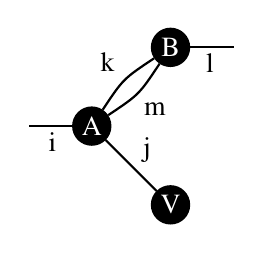
\begin{tikzpicture}[
    dot/.style = {circle, fill, minimum size=#1,
                inner sep=0pt, outer sep=0pt},
    dot/.default = 6pt  % size of the circle diameter 
                    ]  
    \def\dx{0};
    \def\r{0.25cm}
    \def\ax{0}
    \def\ay{0}
    \def\bx{1}
    \def\by{1}
    \def\cx{1}
    \def\cy{-1}
    \node[color=white, fill=black, dot=2*\r] at (\ax+\dx,\ax) (a) {A};
    \node[color=white, fill=black, dot=2*\r] at (\bx+\dx,\by) (b) {B};
    \node[color=white, fill=black, dot=2*\r] at (\cx+\dx,\cy) (c) {V};
    %\draw [black,thick] (\ax+\dx,\ay) .. controls (0.5*\ax+0.5*\bx+\dx+0.2,0.5*\ay+0.5*\by-0.2) .. (\bx+\dx,\by);
    %\draw [black,thick] (\ax+\dx,\ay) .. controls (0.5*\ax+0.5*\bx+\dx-0.2,0.5*\ay+0.5*\by+0.2) .. (\bx+\dx,\by);
    \draw [black,thick] (a) .. controls (0.4, 0.6) .. (b);
    \draw [black,thick] (a) .. controls (0.6, 0.4) .. (b);
    \draw [black,thick] (a) -- (c);
    \draw [black,thick] (a) -- (\ax+\dx-0.8,\ay);
    \draw [black,thick] (b) -- (\bx+\dx+0.8,\by);
    \node[color=black] at (0.5*\ax+0.5*\bx-0.3+\dx,0.5*\ay+0.5\by+0.3) {k};
    \node[color=black] at (0.5*\ax+0.5*\bx+0.3+\dx,0.5*\ay+0.5\by-0.3) {m};
    \node[color=black] at (0.5*\ax+0.5*\cx+\dx+0.2,0.5*\ay+0.5\cy+0.2) {j};
    \node[color=black] at (\ax+\dx-0.5,\ay-0.2) {i};
    \node[color=black] at (\bx+\dx+0.5,\by-0.2) {l};
\end{tikzpicture}}

\end{example}

Here, we want to use a generalized tensor network notation by not restricting the number of times a label appears in the notation,
hence whether an index is a superscript or a subscript makes no sense now.
It is also called einsum, sum-product network or factor graph~\cite{Bishop2006} in some contexts.
The graphical representation of a tensor network in this paper is a hypergraph, where an edge (label) can be shared by an arbitrary number of vertices (tensors).

\begin{example}
$C_{ijk} = A_{jkm} B_{mil} V_{jm}$ is a tensor network, it represents $C_{ijk} = \sum_{ml}A_{jkm} B_{mia} V_{jm}$.
Its hypergraph representation is as the following, where we use different color to annotate different hyperedges.

\centerline{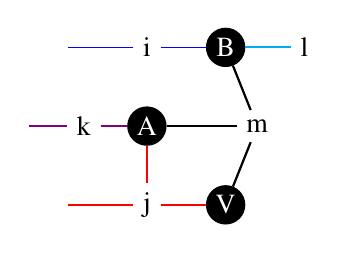
\begin{tikzpicture}[
    dot/.style = {circle, fill, minimum size=#1,
                inner sep=0pt, outer sep=0pt},
    dot/.default = 6pt  % size of the circle diameter 
                    ]  
    \def\dx{0};
    \def\r{0.5cm}
    \def\ax{0}
    \def\ay{0}
    \def\bx{1}
    \def\by{1}
    \def\cx{1}
    \def\cy{-1}
    \node[color=white,fill=black,dot=\r] at (\ax+\dx,\ax) (a) {A};
    \node[color=white,fill=black,dot=\r] at (\bx+\dx,\by) (b) {B};
    \node[color=white,fill=black,dot=\r] at (\cx+\dx,\cy) (v) {V};
    \node at (\ax-0.8,\ay) (k) {k};
    \node at (\bx+0.4,\ay) (m) {m};
    \node at (\ax,\cy) (j) {j};
    \node at (\bx+1,\by) (l) {l};
    \node at (\bx-1,\by) (i) {i};
    \draw[color=blue] (i) -- (b);
    \draw[color=blue] (i) -- (\ax-1,\by);
    \draw[color=cyan,thick] (l) -- (b);
    \draw[color=violet,thick] (k) -- (a);
    \draw[color=violet,thick] (k) -- (\ax-1.5,\ay);
    \draw[color=black,thick] (b) -- (m);
    \draw[color=black,thick] (m) -- (a);
    \draw[color=black,thick] (m) -- (v);
    \draw[color=red,thick] (a) -- (j);
    \draw[color=red,thick] (v) -- (j);
    \draw[color=red,thick] (\ax-1,\cy) -- (j);
\end{tikzpicture}}
\end{example}

In the main text, we stick to the our generalized tensor network notation rather than the traditional notation.
As a note to those who are more familiar with the traditional tensor network representation,
although one can easily translate a generalized tensor network to the equivalent traditional tensor network by adding $\delta$ tensors (a generalization of identity matrix to higher order).
It can sometime increase the contraction complexity of a graph. We have an example demonstrating this point in \App{app:tensorbad}.

\section{Independence polynomial}
One can encode the independence polynomial~\cite{Ferrin2014, Harvey2017} of $G$ to a tensor network.
Independence polynomial is an important graph polynomial that contains the counting information of an independent set problem. It is defined as
\begin{equation}
I(G, x) = \sum_{k=1}^{\alpha(G)} a_k x^k,
\end{equation}
where $a_k$ is the number of independent sets of size $k$ in $G$, and $\alpha(G)$ is the maximum independent set size.
The problem of computing independence polynomial belongs to the complexity class \#P-hard.
A traditional approach to compute independence polynomial rigorusly requires a computing time $O(1.442^n)$~\cite{Ferrin2014}\blue{I am not sure about this complexity, this is baed on the naive analysis of theorem 2.2 in ~\cite{Ferrin2014}}.
%with which computing the independence polynomial for a square lattice of size $30\times 30$ would be impossible.
There are some interests in approximating this polynomial efficiently~\cite{Harvey2018}, but here, we focus on the rigorous approaches.
We encode this polynomial to a tensor network by placing a rank one tensor of size $2$ parametrized by $x_i$ on a vertex $i$
\begin{equation}
    W(x_i)_{s_i} = \left(\begin{matrix}
        1 \\
        x_i
    \end{matrix}\right)_{s_i},\label{eq:wtensor}
\end{equation}
and a rank two tensor of size $2 \times 2$ on an edge $(i,j)$
\begin{equation}
    B_{s_i s_j} = \left(\begin{matrix}
        1  & 1\\
        1 & 0
    \end{matrix}\right)_{s_is_j},\label{eq:btensor}
\end{equation}
where a tensor index $s_i$ is a boolean variable that having the meaning of being 1 if vertex $i$ is in the independent set, 0 otherwise.
It corresponds to a hyperedge in the hypergraph.
The contraction of such a tensor network gives
\begin{equation}
    P(G, \{x_1,\ldots,x_n\}) = \sum\limits_{s_1, s_2, \ldots, s_n = 0}^{1} \prod\limits_{i=1}^n W(x_i)_{s_i} \prod\limits_{(i,j) \in E(G)} B_{s_i s_j},
\end{equation}
where the summation runs over all vertex configurations $\{s_1,\ldots,s_n\}$ and accumulates the product of tensor elements to the scalar output $P$.
We can see an edge tensor represents the restriction on an edge that if both vertices connected by it are included in the set, then such configuration has no contribution to the output.
When we set $x_i = x$, the contraction result corresponds to the independence polynomial.
One can see the connection from the fact that the product over vertex tensor elements gives a factor $x^k$, where $k=\sum_i s_i$ counts the set size, 
and the product over edge tensor elements gives a factor $1$ for a configuration being in an independent set, $0$ otherwise.
One directly benefit of mapping the independent set problem to a tensor network is one can take the advantage of recently developed techniques in tensor network based quantum circuit simulations ~\cite{Gray2021,Pan2021},
where people evaluate a tensor network by pairwise contracting tensors in a heuristic order.
A good contraction order can reduce the time complexity significantly, at the cost of having a space overhead of $O(2^{tw(G)})$.
Here $tw(G)$ is the tree width of the line graph of a tensor network hypergraph, while the line graph of a tensor network hypergraph corresponds to the original graph $G$ that we mapped from.~\cite{Markov2008}
The pairwise tensor contraction also makes it possible to utilize basic linear algebra subprograms (BLAS) functions to speed up our computation for certain tensor element types.

\begin{example}
    Mapping a graph (left) to a tensor network, the resulting tensor network is shown in the right panel.
    In the generalize tensor network's graphical representation, a vertex is mapped to a hyperedge,
    and an edge is mapped to an edge tensor.

    \centerline{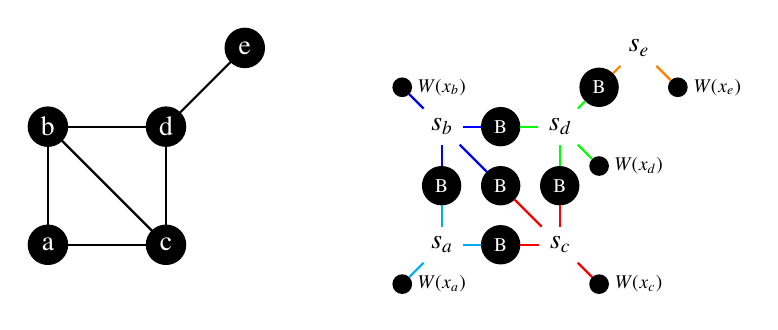
\begin{tikzpicture}[
    dot/.style = {circle, fill, minimum size=#1,
                inner sep=0pt, outer sep=0pt},
    dot/.default = 6pt  % size of the circle diameter 
                    ]  

        \def\dx{0};
        \def\r{0.25cm}
        \filldraw[fill=black] (\dx,0) circle [radius=\r];
        \filldraw[fill=black] (\dx,1.5) circle [radius=\r];
        \filldraw[fill=black] (1.5+\dx,0) circle [radius=\r];
        \filldraw[fill=black] (1.5+\dx,1.5) circle [radius=\r];
        \filldraw[fill=black] (2.5+\dx,2.5) circle [radius=\r];
        \draw [black,thick] (\dx,0) -- (\dx,1.5);
        \draw [black,thick] (\dx,0) -- (1.5+\dx,0);
        \draw [black,thick] (\dx,1.5) -- (1.5+\dx,1.5);
        \draw [black,thick] (1.5+\dx,0) -- (1.5+\dx,1.5);
        \draw [black,thick] (1.5+\dx,0) -- (\dx,1.5);
        \draw [black,thick] (2.5+\dx,2.5) -- (1.5+\dx,1.5);
        \node[color=white] at (\dx,0) {a};
        \node[color=white] at (\dx,1.5) {b};
        \node[color=white] at (1.5+\dx,0) {c};
        \node[color=white] at (1.5+\dx,1.5) {d};
        \node[color=white] at (2.5+\dx,2.5) {e};
        \def\dx{5};
        \def\r{0.25cm}
        \foreach \x/\y/\e in {0.75/0/ac, 0/0.75/ab, 1.5/0.75/cd, 0.75/1.5/bd, 0.75/0.75/bc, 2/2/de}
            \node[color=white,fill=black,dot=2*\r] at (\x+\dx,\y) (\e) {\scriptsize B};
        \foreach \x/\y/\v in {0/0/a, 0/1.5/b, 1.5/0/c, 1.5/1.5/d, 2.5/2.5/e}
            \node[color=black] at (\x+\dx,\y) (\v) {$s_\v$};
        \foreach \x/\y/\v in {-0.5/-0.5/a, -0.5/2.0/b, 2.0/-0.5/c, 2.0/1.0/d, 3.0/2.0/e}
            \node[color=white,fill=black,dot=\r] at (\x+\dx,\y) (\v\v) {};
        \foreach \x/\y/\v in {-0.5/-0.5/a, -0.5/2.0/b, 2.0/-0.5/c, 2.0/1.0/d, 3.0/2.0/e}
            \node[color=black] at (\x+\dx+0.5,\y) {\scriptsize $W(x_\v)$};
        \draw [cyan,thick] (a) -- (aa);
        \draw [cyan,thick] (a) -- (ab);
        \draw [cyan,thick] (a) -- (ac);
        \draw [blue,thick] (b) -- (bb);
        \draw [blue,thick] (b) -- (ab);
        \draw [blue,thick] (b) -- (bc);
        \draw [blue,thick] (b) -- (bd);
        \draw [red,thick] (c) -- (cc);
        \draw [red,thick] (c) -- (ac);
        \draw [red,thick] (c) -- (bc);
        \draw [red,thick] (c) -- (cd);
        \draw [green,thick] (d) -- (dd);
        \draw [green,thick] (d) -- (bd);
        \draw [green,thick] (d) -- (de);
        \draw [green,thick] (d) -- (cd);
        \draw [orange,thick] (e) -- (ee);
        \draw [orange,thick] (e) -- (de);
    \end{tikzpicture}}
    The contraction of this network can be done in a pairwise order.
    \begin{align*}
        &\sum_{s_a,s_b,s_c,s_d,s_e} W(x_a)_{s_a} W(x_b)_{s_b} W(x_c)_{s_c} W(x_d)_{s_d} W(x_e)_{s_e} B_{s_a s_b} B_{s_b s_d} B_{s_a s_c} B_{s_b s_c} B_{s_d s_e}.\\
        =&\sum_{s_b,s_c}\left(\sum_{s_d}\left(\left(\left(\left(\sum_{s_e}B_{s_d s_e}W(x_e)_{s_e}\right) W(x_d)_{s_d}\right) \left(B_{s_bs_d} W(x_b)_{s_b}\right)\right) \left(B_{s_cs_d} W(x_c)_{s_c}\right)\right)\right.\\
        &\phantom{XXX}\left.\left(B_{s_bs_c}\left(\sum_{s_a}B_{s_as_b}\left(B_{s_as_c}W(x_a)_{s_a}\right)\right)\right)\right)\\
        =&1 + x_a + x_b + x_c + x_d + x_e + x_ax_d + x_ax_e + x_cx_e + x_bx_e\\
        =&1+5x+4x^2
    \end{align*}
\end{example}


Before contracting the tensor network and evaluating the independence polynomial numerically, let us first give up thinking $0$s and $1$s in tensors $W(x)$ and $B$ as regular computer numbers such as integers and floating point numbers.
Instead, we treat them as the additive identity and multiplicative identity of a commutative semiring.
A semiring is a ring without additive inverse, while a commutative semiring is a semiring that multiplication commutative.
To define a commutative semiring with addition algebra $\oplus$ and multiplication algebra $\odot$ on a set $R$, the following relations must hold for arbitrary three elements $a, b, c \in R$.
\begin{align*}
(a \oplus b) \oplus c = a \oplus (b \oplus c) & \hspace{5em}\text{$\triangleright$ commutative monoid $\oplus$ with identity $\mymathbb{0}$}\\
a \oplus \mymathbb{0} = \mymathbb{0} \oplus a = a &\\
a \oplus b = b \oplus a &\\
&\\
(a \odot b) \odot c = a \odot (b \odot c)  &   \hspace{5em}\text{$\triangleright$ commutative monoid $\odot$ with identity $\mymathbb{1}$}\\
a \odot  \mymathbb{1} =  \mymathbb{1} \odot a = a &\\
a \odot b = b \odot a &\\
&\\
a \odot (b\oplus c) = a\odot b + a\odot c  &  \hspace{5em}\text{$\triangleright$ left and right distributive}\\
(a\oplus b) \odot c = a\odot c \oplus b\odot c &\\
&\\
a \odot \mymathbb{0} = \mymathbb{0} \odot a = \mymathbb{0}
\end{align*}
The property of being commutative is required here because we want the contraction result independent of the contraction order.
In the following, we show how to obtain the independence polynomial, the maximum independent set size and optimal configurations of a general graph $G$ by designing tensor element types as commutative semirings,
i.e. making the tensor network generic~\cite{Stepanov2014}.
A straight forward approach to evaluate the independence polynomial is treating the tensor elements as polynomials, and evaluate the polynomial directly.
Let us create a polynomial type, and represent a polynomial $a_0 + a_1 x + \ldots + a_k x^k$ as a vector $(a_0, a_1, \ldots, a_k) \in R^k$, e.g. $x$ is represented as $(0, 1)$.
We define the algebra between the polynomials $a$ of order $k_a$ and $b$ of order $k_b$ as
\begin{align}
    \begin{split}
    a \oplus b &= (a_0 + b_0, a_1 + b_1, \ldots, a_{\max(k_a, k_b)} + b_{\max(k_a, k_b)}),\\
    a \odot b &= (a_0 + b_0, a_1b_0 + a_0b_1, \ldots, a_{k_a} b_{k_b}),\\
    \mymathbb{0} &= (),\\
    \mymathbb{1} &= (1).\label{eq:polynomial}
    \end{split}
\end{align}
By contracting the tensor network with polynomial type, the final result is the exact representation of the independence polynomial.
In the program, the multiplication can be evaluated efficiently with the convolution theorem~\cite{Schonhage1971}.
However, this approach suffers from a space overhead that proportional to the maximum independent set size because each polynomial requires a vector of such size to store the factors.
In \App{app:fft}, we provide a fitting based approach to compute the independence polynomial.
One just set $x$ to $\alpha(G)+1$ random values, compute the result and use the polynomial fitting to get the factors.
In this way, we do not have linear overheads in space, however, 
due to fact that countings of different MIS sizes can be different in many orders, 
the round off error dominates the high MIS size region that we are most interested about if we use floating point numbers in computation, 
meanwhile the number easily overflows if we use fixed width integer types.
The big integer type is not an option because big integers with varying width can be very slow and incompatible with graphic processing units (GPU) devices.
Then we want to resort to integer numbers, however, fixed width integer types are often too small to store the counting,
This problem can be solved by introducing finite field algebra $GF(p)$
\begin{align}
\begin{split}
    x ~\oplus~ y &= x+y\pmod p,\\
    x ~\odot~ y &= xy\pmod p,\\
    \mymathbb{0} &= 0,\\
    \mymathbb{1} &= 1.
\end{split}\label{eq:finitefield}
\end{align}
In a finite field algebra, we have the following observations
\begin{enumerate}
    \item One can use Gaussian elimination~\cite{Golub2013} to solve a linear equation \Eq{eq:lineareq}
    because it is a generic function that works for any elements with field algebra.
    The multiplicative inverse of a finite field algebra can be computed with the extended Euclidean algorithm.
    \item Given the remainders of a larger unkown integer $x$ over a set of co-prime integers $\{p_1, p_2, \ldots, p_n\}$,
    $x \pmod {p_1 \times p_2 \times \ldots \times p_n}$ can be computed using the Chinese remainder theorem.
    With this, one can infer big integers from small integers.
\end{enumerate}
With these observations, we developed Algorithm~\ref{alg:finitefield} to compute independence polynomial exactly without introducing space overheads.
In the algorithm, except the computation of Chinese remainder theorem, all computations are done with integers of fixed width $W$.

\begin{algorithm}[!ht]
    \small
    \SetAlgoNoLine
    \LinesNumbered
    Let $P = 1$, vector $X = (0,1,2,\ldots,m)$, matrix $\hat X_{ij} = X_i^j$, where $i,j = 0, 1, \ldots m$\;

    \While{true}{
        compute the largest prime $p$ that $\gcd(p, P) = 1$ and $p \leq 2^W$\;

        compute the tensor contraction on $GF(p)$ and obtain $Y = (y_0, y_1, \ldots , y_m) \pmod p $\;

        $A_p = (a_0, a_1, \ldots, a_m) \pmod p = {\rm gaussian\_elimination}(\hat X, Y \pmod p) $\;

        $A_{P\times p} = {\rm chinese\_remainder}(A_P, A_p)$\;

        \If{$A_P = A_{P \times p}$}{
            \Return $A_P$ \tcp*[l]{converged}
        }
        $P = P \times p$\;
    }\caption{Compute independence polynomial exactly without integer overflow}\label{alg:finitefield}
\end{algorithm}

\subsection{Maximal independence polynomial}
Some times people are interested in knowing maximal solutions to understand why their programs are trapped in a local minimal.
Then they might want to compute the maximal independence polynomial.
Let us denote the neighbour of a vertex $v$ as $N(v)$ and $N[v] = N(v)\cup \{v\}$.
A maximal independent set $I_m$ is an independent sets that there does not exist a vertex $v$ that $N[v] \cap I_m = \emptyset$.
Let us modify the tensor network for computing independence polynomial by adding this restriction.
Instead of defining the restriction on vertices and edges, we define it on $N[v]$
\begin{align}
    T(x_v)_{s_1,s_2,\ldots,s_{|N(v)|},s_v} = \begin{cases}
        s_vx_v & s_1=s_2=\ldots=s_{|N(v)|}=0,\\
        1-s_v& otherwise.\\
    \end{cases}
\end{align}
As an example, for a vertex of degree 2, the resulting rank 3 tensor is
\begin{align}
    T(x_v)=\left(\begin{matrix}
    \left(\begin{matrix}
        0 &1 \\
        1 &1
    \end{matrix}\right)\\
    \left(\begin{matrix}
        x_v &0 \\
        0 &0
    \end{matrix}\right)
    \end{matrix}\right).
\end{align}

We do the same computation as independence polynomial, the coefficients of resulting polynomial gives the counting of maximal independent sets, or the maximal independence polynomial.
The computational complexity of this new tensor network is often larger than the one for computing independence polynomial.
However, in many sparse graphs, this tensor network contraction approach is still much faster than computing the maximal cliques on its complement by applying the Bron-Kerbosch algorithm.

\section{Maximum independent sets and its counting problem}
In the previous section, we focused on computing independence polynomial for a given maximum independent set size $\alpha(G)$, but we didn't mention how to compute this number.
The method we use to compute this quantity is based on the following observations. Let $x=\infty$, the independence polynomial becomes
\begin{equation}
I(G, \infty) = a_k \infty^{\alpha(G)},
\end{equation}
where the lower orders terms disappear automatically. We can define a new algebra as
\begin{align}
\begin{split}
    a_x\infty^x \oplus a_y\infty^y &= \begin{cases}
        (a_x + a_y)\infty^{\max(x,y)}, & x = y\\
        a_y\infty^{\max(x,y)}, & x < y\\
        a_x\infty^{\max(x,y)}, & x > y
    \end{cases}\\
    a_x\infty^x \odot a_y\infty^y &= a_x a_y\infty^{x+y}\\
    \mymathbb{0} &= 0\infty^{-\infty}\\
    \mymathbb{1} &= 1\infty^{0}\label{eq:countingtropical}
\end{split}
\end{align}
In the program, we only store the power $x$ and the corresponding factor $a_x$ that initialized to $1$.
This algebra is the same as the one in ~\cite{Liu2021} for counting spin glass ground states.
If one is only interested in obtaining $\alpha(G)$, he can drop the factor parts, then the new algebra becomes the max-plus tropical algebra~\cite{Maclagan2015,Moore2011}.

\subsection{Sub-optimal solutions}
Some times people are interested in finding sub-optimal solutions efficiently.
We define a truncated polynomial algebra by keeping only largest two factors in the polynomial in \Eq{eq:polynomial}.
\begin{align}
    \begin{split}
    a \oplus b &= (a_{\max(k_a, k_b)-1} + b_{\max(k_a, k_b)-1}, a_{\max(k_a, k_b)} + b_{\max(k_a, k_b)}),\\
    a \odot b &= (a_{k_a-1} b_{k_b}+a_{k_a} b_{k_b-1}, a_{k_a} b_{k_b}),\\
    \mymathbb{0} &= (),\\
    \mymathbb{1} &= (1).\label{eq:max2poly}
    \end{split}
\end{align}
%By changing the factors to sets, and plus and multiplication operations on factors to set union and product, one can get all suboptimal solutions too.
In the program, we need a data structure that contains three fields, the largest order $k$ and factors for two largest orders $a_k$ and $a_{k-1}$.

\section{Enumerating configurations}
One may also want to obtain all solutions, it can be achieved replacing the factors with a set of solutions,
We design a new element type having the following algebra
\begin{align}
\begin{split}
    s \oplus t &= s \cup t\\
    s \odot t &= \{\sigma \lor^\circ \tau | \sigma \in s, \tau \in t\}\\
    \mymathbb{0} &= \{\}\\
    \mymathbb{1} &= \{0^{\otimes n}\}
\end{split}\label{eq:set}
\end{align}
where $\lor^\circ$ is the Hadamard logic or operation over two bit strings, which means joining of two local configurations.
The variable $x$ in the vertex tensor is initialized to $x_i = \{\boldsymbol{e}_{i}\}$,
where $\boldsymbol{e}_i$ is a one hot vector of size $|G|$.
As an example, if we want to enumerate all maximum independent sets, we can use the above set as the factors in \Eq{eq:countingtropical}.
We get the following new algebra.
\begin{align}
\begin{split}
    s_x\infty^x \oplus s_y\infty^y &= \begin{cases}
        (s_x \cup s_y)\infty^{\max(x,y)}, & x = y\\
        s_y\infty^{\max(x,y)}, & x < y\\
        s_x\infty^{\max(x,y)}, & x > y
    \end{cases},\\
    s_x\infty^x \odot s_y\infty^y &= \{\sigma \lor^\circ \tau | \sigma \in s_x, \tau \in s_y\}\infty^{x+y},\\
    \mymathbb{0} &= \{\}\infty^{-\infty},\\
    \mymathbb{1} &= \{0^{\otimes n}\}\infty^{0},
\end{split}
\end{align}
One can easily check if the factor algebra is a commutative semiring,
when we use the above algebra as factors of independence polynomials, the resulting algebra is also a commutative semiring.
If one is only interested in obtaining a single configuration, one can also just keep a single configuration to save the computational effort.
We arrive at a new algebra defined on bit strings.
%We leave this as an exercise for readers.

\iffalse
\begin{align}
\begin{split}
    \sigma_x\infty^x \oplus \sigma_y\infty^y &= \begin{cases}
        {\rm select}(\sigma_x, \sigma_y)\infty^{\max(x,y)}, & x = y\\
        \sigma_y\infty^{\max(x,y)}, & x < y\\
        \sigma_x\infty^{\max(x,y)}, & x > y
    \end{cases},\\
    \sigma_x\infty^x \odot \sigma_y\infty^y &= (\sigma_x \lor^\circ \sigma_y)\infty^{x+y},\\
    \mymathbb{0} &= 1^{\otimes n}\infty^{-\infty},\\
    \mymathbb{1} &= 0^{\otimes n}\infty^{0},
\end{split}
\end{align}
\fi
\begin{align}
\begin{split}
    \sigma \oplus \tau &= {\rm select}(\sigma, \tau)\\
    \sigma \odot \tau &= (\sigma\lor^\circ \tau),\\
    \mymathbb{0} &= 1^{\otimes n},\\
    \mymathbb{1} &= 0^{\otimes n},
\end{split}\label{eq:singleconfig}
\end{align}
where the \texttt{select} function picks one of $\sigma_x$ and $\sigma_y$ by some criteria to make the algebra commutative and associative, e.g. by their integer values.
In practise, one can just pick randomly from them, then the program will output one of the configurations randomly.

\subsection{Bounding the enumeration space}
When one uses the set algebra in \Eq{eq:set} to represent the factors in \Eq{eq:countingtropical} for enumerating all optimum configurations, he will find the program stores more than necessary intermediate configurations and cause significant overheads in space.
To speed up the computation, we use $\alpha(G)$ to bound the searching space.
We first compute the value of $\alpha(G)$ with tropical numbers and cache all intermediate tensors.
Then we compute a boolean masks for each cached tensor, where we use a boolean true to represent a tensor element having contribution to the maximum independent set (i.e. with a non-zero gradient) and boolean false otherwise.
Finally, we perform masked matrix multiplication using the new element type with the above algebra for obtaining all configurations.
Notice that these masks are in fact tensor elements with non-zero gradients with respect to MIS size, we compute these masks by back propagating gradients.
To derive the backward rule for tensor contraction,
we first reduce the problem to finding the backward rule of a tropical matrix multiplication $C = A B$,
where we have the following inequality
\begin{align}
    A_{ij} \odot B_{jk} &\leq C_{ik}.
\end{align}
Here is $\leq$ on tropical numbers are same as regular algebra.
The tropical multiplication $\odot$ is the same as the regular $+$, then
one can move $B_{ik}$ to the right hand side and get
\begin{align}
    A_{ij} &\leq C_{ik} \odot B_{jk}^{\circ -1}
\end{align}
where the tropical multiplicative inverse is defined as the additive inverse of the regular algebra.
The inequality still holds if we take the minimum over $k$
\begin{align}
    \begin{split}
    A_{ij} &\leq \min_{k}(C_{ik} \odot B_{jk}^{\circ -1}) = (\oplus_{k} (C_{ik}^{-1} \odot B_{jk}))^{\circ -1}.
    \end{split}
\end{align}
On the right hand side, we transformed the operation into a tropical matrix multiplication so that we can utilize the fast tropical BLAS routines.
The equality holds if and only if element $A_{ij}$ has contribution to $C$ (i.e. has non-zero gradient).
Let the gradient mask for $C$ being $\overline C$, the backward rule for gradient masks reads
\begin{align}
\overline{A}_{ij} = \delta(A_{ij}, ((C^{\circ-1} \circ \overline C )B^T)_{ij}^{\circ -1}),
\end{align}
where ${}^{\circ -1}$ is the Hadamard inverse, $\circ$ is the Hadamard product, boolean false is treated as tropical zero and boolean true is treated as tropical one.
This rule defined on matrix multiplication can be easily generalized to tensor contraction by replacing the matrix multiplication between $C^{\circ-1} \circ \overline C$ and $B^T$ by a tensor contraction.~\cite{} \blue{maybe add an appendix?}  % my blog

\section{Tropical tensors for automated branching}\blue{$?$}
% check http://www.tcs.rwth-aachen.de/independentset/ for more rules
Branching rules can be automatically discovered by contracting the tensor network on a subgraph $R \subseteq G$ with tropical numbers as its element type.
Let $C$ be the set of boundary vertices defined as $C := \{u | u\in R \land (\exists v \in (G\backslash R) \land {\rm adj}(u, v))\}$, then the rank of the resulting tensor $A$ is $|C|$.
Here, we use ${\rm adj}(u, v)$ to denote two vertices $u$ and $v$ are adjacent to each other.
Each tensor entry $A_{\sigma}$ is a local maximum independent set size for the fixed boundary configuration $\sigma \in \{0,1\}^{|C|}$.
Suppose our goal is to find the maximum independent set size,
then this tensor can be further ``compactified'' by removing some entries.
To determine which entry can be removed, let us define a relation of \textit{less restrictive} as
\begin{align}
(\sigma_a \prec \sigma_b) := (\sigma_a \neq \sigma_b) \land (\sigma_a \leq^\circ \sigma_b)
\end{align}
where $\leq^\circ$ is the Hadamard less or equal to operation.

\begin{definition}
A tensors $A$ is \textit{MIS-compact} if
\begin{align}
\forall{\sigma_b}\neg \exists{\sigma_a}(\sigma_a \prec \sigma_b) \land (A_{\sigma_a} \geq A_{\sigma_b})\label{eq:compactifying}.
\end{align}
\end{definition}

If we remove such $A_{\sigma_b}$, the contraction over the whole graph is guaranteed to give the same maximum independent set size.
It can be seen by considering two entries with the same local maximum independent set sizes and different boundary configurations as shown in \Fig{fig:compactifying} (a) and (b).
If we have $\sigma_b \cup \overline{\sigma_b}$ being one of the solutions for maximum independent sets in $G$, then $\sigma_a \cup \overline{\sigma_b}$ is another solution giving the same $\alpha(G)$.
Hence, we can remove entry $A_{\sigma_b}$ safely.
%among boundary configurations with equal local maximum independent sizes,
%we only retain those least restrictive (less ones at the boundary) to exterial configurations.

\begin{figure}
    \centering
    \includegraphics[width=0.8\textwidth, trim={5cm 4cm 5cm 4cm}, clip]{compressionrule.pdf}
    \caption{Two configurations with the same local independent size $A_{\sigma_a} = A_{\sigma_b} = 3$ and different boundary configurations (a) $\sigma_a=\{001\}$ and (b) $\sigma_b = \{101\}$, where black nodes are $1$s (in the independent set) and white nodes are $0$s (not in the independent set).}\label{fig:compactifying}
\end{figure}

\begin{theorem}
    A MIS-compact tropical tensor can not be further reduce without gloal information, i.e. any of its non-zero entries can produce the only global optimal solution given a proper environment.
\end{theorem}

\begin{proof}
    %Given $A_\{\sigma_a}$ is better than $A_\{\sigma_b\}$, any exterior configuration $\overline{\sigma}$ making $\overline{\sigma} \cup \sigma_b$ a global maximum independent set also makes $\overline{\sigma} \cup \sigma_a$ a maximum independent set.
    Let us prove it by showing for any $\sigma$ in a MIS-compact tropical tensor of a subgraph $R$, there exists a parent graph $G$ that $R\subseteq G$ and $\sigma$ is the boundary configuration that gives the only maximum independent set.
    Let $A$ be a tropical tensor, and an entry of it being $A_{\sigma}$, where $\sigma$ is the boundary configuration.
    Let us construct a graph $G$ such that for a vertex $v \in C$, if $\sigma_v=1$, we connect it with two vertices $u, w \in G \backslash R$ that ${\rm adj}(v, u) \land {\rm adj}(u, w) \land \neg{\rm adj}(v, w)$. Otherwise, we attach infinite many disconnected neighbors to $v$.

    \centerline{\includegraphics[width=0.35\textwidth, trim={0cm 2cm 5cm 0cm}, clip]{proofoptimal.pdf}}
    Then we have the maximum independent set size $\alpha(G,\sigma) = A_{\sigma} + \infty (|C|-\sum_{v=1}^{|C|}\sigma_v) + \sum_{v=1}^{|C|} 1-\sigma_v$.
    Let us assume there exists another configuration $\tau$ that generating the same or better maximum independent set size $\alpha(G, \tau) \geq \alpha(G, \sigma)$.
    Then we have $\tau \prec \sigma$, otherwise it will loss infinite contribution from the environment.
    For such a $\tau$, we have $A_\tau < A_\sigma$, otherwise $A_\sigma \prec A_\tau$ contradicts with $A$ being MIS-compact.
    Finally, we have $\alpha(G,\tau) = \infty (|C|-|\sigma|) + A_{\tau} + \sum_{v=1}^{|C|} 1-\sigma_v < \alpha(G,\sigma)$, hence $\sigma$ is the only boundary configuration that gives the maximum independent set for this graph.
\end{proof}

\subsection{The tensor network compactification detects branching rules automatically}
Almost all branching rules are based on the same idea of analysing a local subgraph induced by a vertex $v$
by including its neighbourhoods,
and keep only the configurations that has the potential to produce the only maximum independent set.
Since an MIS-compact tensor is optimal, by analysing the correlation of vertex configurations on the resulting tensor for the $k$-th neighbourhood $N^k[v]$, one can discover the optimal branching vector automatically.
In the following, we are going to introduce several important rules for branching in the literature and show how it is connected to our tensor formulation.

\begin{corollary}\label{rule:one} % basic
  If a vertex $v$ is in an independent set $I$, then none of its Neighbors can be in $I$.
On the other hand, if $I$ is a maximum (and thus maximal) independent set,
and thus if $v$ is not in $I$ then at least one of its Neighbors is in $I$.
\end{corollary}

Contract $N[v]$ and the resulting tensor $A$ has a rank $|N(v)|$. Each tensor entry $A_{\sigma}$ corresponds to a locally maximized independent set size with fixed boundary configuration $\sigma \in \{0, 1\}^{|N(v)|}$.
If the boundary configuration is a bit string of 0s, $\sigma_v$ will takes value $1$ to maximize the local independent set size.

\centerline{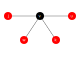
\includegraphics[width=0.4\columnwidth,trim={0 3.5cm 0 1cm},clip]{../notebooks/basic.pdf}}

After contracting $N[v]$, $v$ becomes an internal degree of freedom.
Applying tensor compactification rule \Eq{eq:compactifying}, the resulting rank 4 tropical tensor is

\begin{align}
    T_{juwk} = \left(\begin{matrix}
        \left(\begin{matrix}
        ~~~~1 & -\infty \\
        -\infty & ~~~~2
        \end{matrix}\right)_{ju}&
        \left(\begin{matrix}
        -\infty & ~~~~2 \\
        ~~~~2 & ~~~~3
        \end{matrix}\right)_{ju}\\
        \left(\begin{matrix}
        -\infty & ~~~~2 \\
        ~~~~2 & ~~~~3
        \end{matrix}\right)_{ju} &
        \left(\begin{matrix}
        ~~~~2 & ~~~~3 \\
        ~~~~3 & ~~~~4
        \end{matrix}\right)_{ju}
    \end{matrix}\right)_{wk},
\end{align}
where we use ``-'' to denote an entry is forbidden.
If we use sets for counting, one can check all configurations too. The resulting polynomial tensor is
\begin{align}
    P_{juwk} = \left(\begin{matrix}
        \left(\begin{matrix}
        1+x_v & - \\
        - & ~~x_jx_u
        \end{matrix}\right)_{ju}&
        \left(\begin{matrix}
        - & x_ux_k \\
        ~~~~x_jx_k & ~~~~x_ux_jx_k
        \end{matrix}\right)_{ju}\\
        \left(\begin{matrix}
        - & x_wx_u \\
        x_wx_j & x_wx_jx_u
        \end{matrix}\right)_{ju} &
        \left(\begin{matrix}
        x_wx_k & x_wx_kx_u \\
        x_wx_kx_j & x_jx_ux_wx_k
        \end{matrix}\right)_{ju}
    \end{matrix}\right)_{wk}.
\end{align}

By studying the correlation between vertex variables, one can easily see $x_v$ does not co-exist with other vertex variables.
These anti-correlation determines possible branching vectors in the maximum independent set problem.
It is easier to see if we list the set of optimal solutions as
\begin{align}
    \begin{split}
    S_{juwkv} = \{&00001, 10001, 01010, 10010, 11010, 10100,\\&01100, 11100, 00110, 01110, 10110, 11110\}.
    \end{split}
\end{align}
%If we denote the effective branching number of contracting the local degrees of freedoms as $\left|\{A_{\sigma} \neq \mymathbb{0}\right|\sigma \in \{0, 1\}^{|C|}\}|/2^{|R|}$.
%The effective branching value is $11^{1/5} \approx 1.6154$, which is larger than the branching number $\tau(1, 5) \approx 1.3247$.
%It does not mean the tropical tensor does not find all the branches, if we contract $N^2[v]$.
The branching vector $(1,5)$ gives a branching number $\tau(1, 5) \approx 1.3247$

\begin{corollary}[mirror rule] % 2.7
For some $v \in V$, a node $u \in N^2(v)$ is called mirror of $v$, if $N(v) \backslash N(u)$ is a clique. We denote the set of of a node $v$ mirrors~\cite{Fomin2013} by $M(v)$.
Let $G = (V, E)$ be a graph and $v$ a vertex of $G$. Then
\begin{equation}
\alpha(G) = \max(1 + \alpha(G \backslash N[v]), \alpha(G \backslash (M(v) \cup \{v\})).
\end{equation}
\end{corollary}

This rule states that if $v$ is not in $M$, there exists an MIS $I$ that $M(v)\notin I$.
otherwise, there must be one of $N(v)$ in the MIS (\textit{local maximum rule}).
Although this statement involves $N(u)$, however, deriving this rule only requires information upto second neighbourhood of $v$.
If $w$ is in $I$, then none of $N(v) \cap N(w)$ is in $I$, then there must be one of node in the clique $N(v)\backslash N(w)$ in $I$ (\textit{local maximum rule}),
since clique has at most one node in the MIS, by moving the occupied node to the interior, we obtain a ``better'' solution.
%Hence, the \textit{least restrictive principle} captures the mirror rule.
In the following example, since $u\in N^2(v)$ and $N(v) \backslash N(u)$ is a clique, $u$ is a mirror of $v$.

\centerline{\includegraphics[width=0.4\columnwidth,trim={0 3.5cm 0 1cm},clip]{../notebooks/mirror.pdf}}

After contracting $N[v]\cup u$, $v$ becomes an internal degree of freedom.
Applying tensor compactification rule \Eq{eq:compactifying}, the resulting rank 4 tropical tensor is

\begin{align}
    T_{juwk} = \left(\begin{matrix}
        \left(\begin{matrix}
        ~~~~1 & ~~~~2 \\
        ~~~~\cancel{1} & ~~~~\cancel{2}
        \end{matrix}\right)_{ju}&
        \left(\begin{matrix}
        ~~~~\cancel{1} & -\infty \\
        ~~~~2 & -\infty
        \end{matrix}\right)_{ju}\\
        \left(\begin{matrix}
        ~~~~\cancel{1} & ~~~~\cancel{2} \\
        -\infty & -\infty
        \end{matrix}\right)_{ju} &
        \left(\begin{matrix}
        -\infty & -\infty \\
        -\infty & -\infty
        \end{matrix}\right)_{ju}
    \end{matrix}\right)_{wk},
\end{align}
where entries stroked through are removed by compactification. The corresponding polynomial tensor is

\begin{align}
    P_{juwk} = \left(\begin{matrix}
        \left(\begin{matrix}
        1+x_v & x_u+x_ux_v \\
        ~~~~~~~\cancel{} & ~~~~~~~~~~~~~\cancel{}\\
        \end{matrix}\right)_{ju}&
        \left(\begin{matrix}
        ~~~~\cancel{} & - \\
        x_jx_k & -
        \end{matrix}\right)_{ju}\\
        \left(\begin{matrix}
        ~~~~~~~\cancel{} & ~~~~~~~~~~~~~\cancel{} \\
        ~~~~~~~- & ~~~~~~~~~~~~~-
        \end{matrix}\right)_{ju} &
        \left(\begin{matrix}
        ~~~~- & - \\
        ~~~~- & -
        \end{matrix}\right)_{ju}
    \end{matrix}\right)_{wk}.
\end{align}
One can see $w$, as a mirror of $v$ does not appear in the maximum independent set after compactification.

%In this case, the effective branching number is $3^{1/5}\approx 1.2457$,
%which is smaller than the branching number $\tau(4, 2) = 1.2721$ by simply applying the mirror rule.
\begin{align}
    \begin{split}
    S_{juwkv} = \{&00001, 01001, 10010\}.
    \end{split}
\end{align}

\begin{corollary}[satellite rule] % satellite rule
Let $G$ be a graph, $v \in V$. A node $u \in N^2(v)$ is called satellite~\cite{Kneis2009} of $v$, if there is some $u' \in N(v)$ such that $N[u'] \backslash N[v] = \{u\}$.
The set of satellites of a node $v$ is denoted by $S(v)$, and we also use the notation $S[v] := S(v) \cup {v}$. Then 
\begin{equation}
\alpha(G) = \max\{\alpha(G \backslash \{v\}), \alpha(G \backslash N[S[v]]) + |S(v)| + 1\}.
\end{equation}
\end{corollary}

This rule can be capture by contracting $N[v] \cup S(v)$.
In the following example, since $u \in N^2(v)$ and $w \in N(v)$ satisfies $N[w] \backslash N[v] = \{u\}$, $u$ is a satellite of $v$.

\centerline{\includegraphics[width=0.4\columnwidth,trim={0 3.5cm 0 1cm},clip]{../notebooks/satellite.pdf}}

After contracting $N[v] \cup u$, both $v$ and $w$ become internal degrees of freedoms.
Applying tensor compactification rule \Eq{eq:compactifying}, the resulting rank 3 polynomial tensor is
\iffalse
\begin{align}
    T_{juk} = \left(\begin{matrix}
        \left(\begin{matrix}
        ~~~~1 & ~~~~2 \\
        ~~~~2 & ~~~~\cancel{2}
        \end{matrix}\right)_{ju}\\
        \left(\begin{matrix}
        ~~~~\cancel{1} & -\infty \\
        ~~~~\cancel{2} & -\infty
        \end{matrix}\right)_{ju}
    \end{matrix}\right)_{k}.
\end{align}
\fi

\begin{align}
    P_{juk} = \left(\begin{matrix}
        \left(\begin{matrix}
        1+x_w+x_v & x_u + x_ux_v \\
        x_j+x_wx_j & ~~~~~~~~~~~~\cancel{}
        \end{matrix}\right)_{ju}\\
        \left(\begin{matrix}
        ~~~~~~~~~~~~~~~~\cancel{} & ~~~~~~~~~~~~~~~- \\
        ~~~~~~~~~~~~~~~~\cancel{} & ~~~~~~~~~~~~~~~-
        \end{matrix}\right)_{ju}
    \end{matrix}\right)_{k}.
\end{align}

By choosing one of the optimal configurations in each entry,
we can see the satellite rule of either ${v, u} \in I$ or $v \notin I$ is satisfied.

\begin{align}
    \begin{split}
    S_{juwkv} = \{&\{00100,00001\}, 10100, 01001\}.
    \end{split}
\end{align}
%In this case, the effective branching number is $3^{1/5}\approx 1.2457$. 

%We can use the conditional entropy to discover branching rules automatically. 
%Let us take one best configuration a time from each entry of the compact polynomial matrix,
%and denote the resulting configuration set as $S$.
%The conditional entropy matrix here can be defined as
%\begin{align}
%    C_{uv} = H(s_u|s_v)
%\end{align}
%when two variables are strongly correlated to each other, the corresponding entry should be zero.

\subsection{gadget design}\blue{$\times$}

Suppose we have a local structure as the following.

\centerline{\begin{tikzpicture}[scale=1.0]
    \def\r{0.2}
    \foreach \x/\y [count=\i] in {0.17/0.5,0.83/0.5,0.5/0.67,0.5/0.33}
        \node[fill=red,circle,radius=\r] at (\x*8, \y*8) (\i) {};
    \draw (1) -- (2);
    \draw (3) -- (4);
\end{tikzpicture}}


Contract this local structure gives the tropical tensor

\begin{align}
    \left(\begin{matrix}
        \left(\begin{matrix}
            ~~~~0 & ~~~~1\\
            ~~~~1 & ~~~~2
        \end{matrix}\right) &
        \left(\begin{matrix}
            ~~~~1 & -\infty\\
            ~~~~2 & -\infty
        \end{matrix}\right) \\
        \left(\begin{matrix}
            ~~~~1 & ~~~~2\\
            -\infty & -\infty
        \end{matrix}\right) &
        \left(\begin{matrix}
            ~~~~2 & -\infty\\
            -\infty & -\infty
        \end{matrix}\right)
    \end{matrix}\right).
\end{align}

The following gadget is equivalent to the above diagram up to a constant $2$.

\centerline{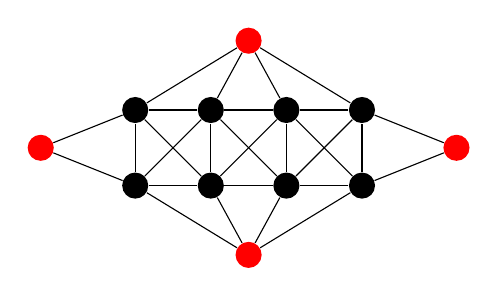
\begin{tikzpicture}
    \def\nodes{(0.5, 0.33), (0.17, 0.5), (0.5, 0.67), (0.83, 0.5), (0.32, 0.44), (0.44, 0.44), (0.56, 0.44), (0.68, 0.44), (0.32, 0.56), (0.44, 0.56), (0.56, 0.56), (0.68, 0.56)}
    \def\edges{(1, 5), (1, 6), (1, 7), (1, 8), (2, 5), (2, 9), (3, 9), (3, 10), (3, 11), (3, 12), (4, 8), (4, 12), (5, 6), (5, 9), (5, 10), (6, 7), (6, 9), (6, 10), (6, 11), (7, 8), (7, 10), (7, 11), (7, 12), (8, 11), (8, 12), (9, 10), (10, 11), (11, 12)}
    \def\r{0.2}
    \foreach \p [count=\i] in \nodes{
        \parsept{\x}{\y}{\p}
        \pgfmathparse{((\x<0.2 || \x>0.8 || \y<0.35 || \y>0.65) ? 1 : 0)}
        \ifnum\pgfmathresult>0
            \node[fill=red,circle,radius=\r] at (\x*8, \y*8) (\i) {};
        \else
            \node[fill,circle,radius=\r] at (\x*8, \y*8) (\i) {};
        \fi
    }
    \foreach \e [count=\i] in \edges{
        \parsept{\x}{\y}{\e}
        \draw (\x) -- (\y);
    }
\end{tikzpicture}}

\begin{align}
    \left(\begin{matrix}
        \left(\begin{matrix}
            ~~~~2 & ~~~~3\\
            ~~~~3 & ~~~~4
        \end{matrix}\right) &
        \left(\begin{matrix}
            ~~~~3 & ~~~~3\\
            ~~~~4 & ~~~~4
        \end{matrix}\right) \\
        \left(\begin{matrix}
            ~~~~3 & ~~~~4\\
            ~~~~2 & ~~~~3
        \end{matrix}\right) &
        \left(\begin{matrix}
            ~~~~4 & ~~~~4\\
            ~~~~3 & ~~~~4
        \end{matrix}\right)
    \end{matrix}\right)
    \xrightarrow[\text{compactify, -2}]{}
    \left(\begin{matrix}
        \left(\begin{matrix}
            ~~~~0 & ~~~~1\\
            ~~~~1 & ~~~~2
        \end{matrix}\right) &
        \left(\begin{matrix}
            ~~~~1 & ~~~~\cancel{1}\\
            ~~~~2 & ~~~~\cancel{2}
        \end{matrix}\right) \\
        \left(\begin{matrix}
            ~~~~1 & ~~~~2\\
            ~~~~\cancel{0} & \cancel{1}
        \end{matrix}\right) &
        \left(\begin{matrix}
            ~~~~2 & ~~~~\cancel{2}\\
            ~~~~\cancel{1} & ~~~~\cancel{2}
        \end{matrix}\right)
    \end{matrix}\right)
\end{align}

We can see these two subgraphs produce exactly the same compact tensor.
When we replace the original tensor with this gadget, the solution.

\section{Benchmarks and case study}
We run a sequetial program benchmark on CPU Intel(R) Core(TM) i5-10400 CPU @ 2.90GHz, and show the results bellow.
\begin{figure}
    \centering
    \includegraphics[width=0.8\textwidth, trim={0cm 0cm 0cm 0cm}, clip]{benchmark.pdf}
    \caption{Benchmark results for computing different properties with different element types.
The right axis is only for the dashed line.
    }\label{fig:benchmark}
\end{figure}
Tensor network contraction is parallelizable. When the element type is immutable, one can just upload the data to GPU to enjoy the speed up.

\section{Discussion}
We introduced in the main text how to compute the independence polynomial, maximum independent set and optimal configurations,
derived the backward rule for tropical tensor network to bound the search of solution space.
%And, we also discussed how to use @tensor network to study the local properties of a graph.
Although many of these properties are global,
we can encode it to different tensor element types as commutative semirings.
The power of tensor network's is not limited to the indenepent set problem, in \App{app:otherproblems} we show how to map matching problem and k-coloring to a tensor network.
Here, we want to discuss more from the programming perspective.
We show some of the Julia language~\cite{Bezanson2012} implementations in Appendix \ref{sec:technical}, you will find it being surprisingly short.
What we need to do is just defining two operations $\oplus$ and $\odot$ and two special elements $\mymathbb{0}$ and $\mymathbb{1}$.
The style that we program is called generic programming,
meaning one can feed different data types into a same program, and the program will compute the result with a proper performance.
In C++, users can use templates for such a purpose.
We chose Julia because its just in time compiling is very powerful that it can generate fast code dynamically for users.
Elements of fixed size, such as the finite field algebra, truncated polynomial, tropical number and tropical number with counting or configuration field used in the main text can be inlined in an array.
Furthermore, these inlined arrays can be upload to GPU devices for faster generic matrix multiplication implemented in CUDA.jl~\cite{Besard2018}.

\begin{table}[h!]\centering
\begin{minipage}{0.9\columnwidth}
\ra{1.3}
    \scalebox{1.0}{
        \begin{tabularx}{\textwidth}{bb}\toprule
            \hline
            \textbf{element type}     & \textbf{purpose} \\
            {regular number}     & {counting all indenepent sets} \\
            {tropical number} (\Eq{eq:countingtropical})    & {finding the maximum independent set size} \\
            {tropical number with counting} (\Eq{eq:countingtropical})     & {finding both the maximum independent set size and its degeneracy} \\
            {tropical number with configurations} (\Eq{eq:singleconfig})     & {finding the maximum independent set size and one of the optimal configurations} \\
            {tropical number with sets} (\Eq{eq:set})    & {finding the maximum independent set size and all optimal configurations} \\
            {polynomial} (\Eq{eq:polynomial})     & {computing the indenpendence polynomials exactly} \\
            {truncated polynomial} (\Eq{eq:max2poly})     & {counting the suboptimal independent sets} \\
            {complex number}     & {fitting the indenpendence polynomials with fast fourier transformation} \\
            {finite field algebra} \Eq{eq:finitefield}    & {fitting the indenpendence polynomials exactly using number theory} \\
            \bottomrule
        \end{tabularx}
    }
    \caption{Tensor element types used in the main text and their purposes.}\label{tbl:generictypes}
\end{minipage}
\end{table}

\section*{Acknowledgments}
We would like to acknowledge Sepehr Ebadi, Maddie Cain and Leo Zhou for popping up inspiring questions,
their questions are the driving force of this project.
Thank Chris Elord for helping us writting the fastest matrix multiplication libary for GEMM, TropicalGEMM.jl, he is a remarkable guy!
\blue{funding information}

\bibliographystyle{siamplain}
\bibliography{refs}

\appendix

\section{Technical guide}\label{sec:technical}
\begin{description}
	\item[OMEinsum] a package for the \texttt{einsum} function,
	\item[OMEinsumContractionOrders] a package for finding the optimal contraction order for the \texttt{einsum} function \\ \href{https://github.com/Happy-Diode/OMEinsumContractionOrders.jl}{https://github.com/Happy-Diode/OMEinsumContractionOrders.jl},
	\item[TropicalGEMM] a package for efficient tropical matrix multiplication (compatible with OMEinsum),
	\item[TropicalNumbers] a package providing tropical number types and tropical algebra, one o the dependency of TropicalGEMM,
	\item[LightGraphs] a package providing graph utilities, like random regular graph generator,
	\item[Polynomials] a package providing polynomial algebra and polynomial fitting,
	\item[Mods and Primes] packages providing finite field algebra and prime number generators.
\end{description}

One can install these packages by opening a Julia REPL, type \colorbox{lightgray}{\texttt{]}} to enter the \texttt{pkg>} mode and type, e.g.
\begin{lstlisting}
pkg> add OMEinsum LightGraphs Mods Primes FFTW Polynomials TropicalNumbers
\end{lstlisting}

It may surprise you that the Julia implementation of algorithms introduced in the paper is so short that except the bounding and sparsity related parts,
all are contained in this appendix. After installing required packages, one can open a Julia REPL and copy the following code into it.

\lstinputlisting[breaklines]{../democode/demo.jl}

In the above examples, the configuration enumeration is very slow, one should use the optimal MIS size for bounding as decribed in the main text.
We will not show any example about implementing the backward rule here because it has approximately 100 lines of code.
Please checkout our GitHub repository \href{https://github.com/Happy-Diode/NoteOnTropicalMIS}{https://github.com/Happy-Diode/NoteOnTropicalMIS}.

\section{Why not introducing $\delta$ tensors}\label{app:tensorbad}

Given a graph

\centerline{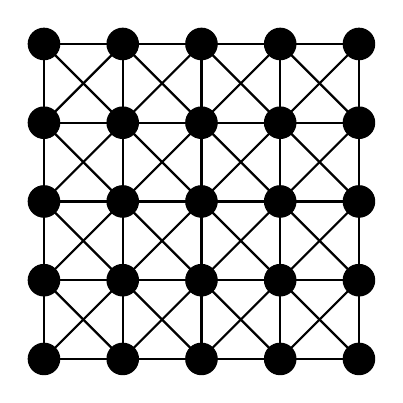
\begin{tikzpicture}
    \def\r{0.2}
    \foreach \x in {1,...,5}
        \foreach \y in {1,...,5}
            \filldraw[fill=black] (\x,\y) circle [radius=\r];
    \foreach \x in {1,...,5}
        \foreach \y in {1,...,4}{
            \draw [black,thick] (\x,\y) -- (\x,\y+1);
            \draw [black,thick] (\y,\x) -- (\y+1,\x);
        }
    \foreach \x in {1,...,4}
        \foreach \y in {1,...,4}{
            \draw [black,thick] (\x,\y) -- (\x+1,\y+1);
            \draw [black,thick] (\y+1,\x) -- (\y,\x+1);
        }
\end{tikzpicture}}

Its traditional tensor network representation with $\delta$ tensors is

\centerline{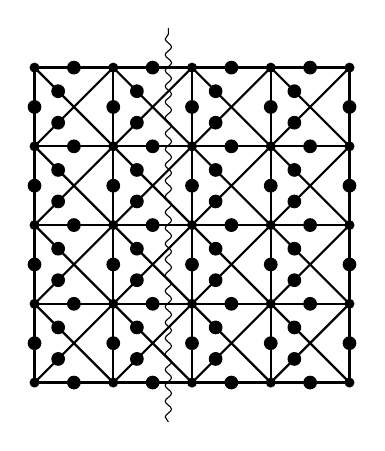
\begin{tikzpicture}
    \def\r{0.08}
    \def\a{0.1}
    \foreach \x in {1,...,5}
        \foreach \y in {1,...,5}
            \filldraw[fill=black] (\x,\y) circle [radius=0.7*\r];
    \foreach \x in {1,...,5}
        \foreach \y in {1,...,4}{
            \filldraw[fill=black] (\x,\y+0.5) circle [radius=\r];
            \filldraw[fill=black] (\y+0.5,\x) circle [radius=\r];
            \draw [black,thick] (\x,\y) -- (\x,\y+1);
            \draw [black,thick] (\y,\x) -- (\y+1,\x);
        }
    \foreach \x in {1,...,4}
        \foreach \y in {1,...,4}{
            \filldraw[fill=black] (\x+0.3,\y+0.3) circle [radius=\r];
            \filldraw[fill=black] (\y+0.3,\x+0.7) circle [radius=\r];
            \draw [black,thick] (\x,\y) -- (\x+1,\y+1);
            \draw [black,thick] (\y+1,\x) -- (\y,\x+1);
        }
    \tikzset{decoration={snake,amplitude=.4mm,segment length=2mm,
                    post length=0mm,pre length=0mm}}
    \draw [decorate] (2.7, 0.5) -- (2.7, 5.5);
\end{tikzpicture}}
where a small circle on an edge is a diagonal tensor. Its rank is $8$ in the bulk. If we contract this tensor network in a naive column-wise order, the maximum intermediate tensor is approximately $3L$, giving a space complexity $\approx 2^{3L}$.
If we treat it as the following generalized tensor network

\centerline{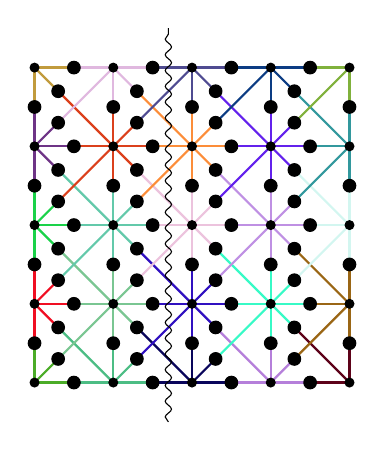
\begin{tikzpicture}
    \def\r{0.08}
    \def\a{0.07}
    \def\L{0.6}
    \def\l{0.1}
    \def\sql{0.24}
    \pgfmathsetseed{2}
    \foreach[evaluate={\cr=0.1+0.5*Mod(\x,2)}] \x in {1,...,5}
        \foreach[evaluate={\cg=0.1+0.3*Mod(\y,2); \cy=0.5-0.5*Mod(\y,2)}] \y in {1,...,5}{
            \edef\R{\pdfuniformdeviate 255}
            \edef\G{\pdfuniformdeviate 255}
            \edef\B{\pdfuniformdeviate 255}
            \xdefinecolor{MyColor}{RGB}{\R,\G,\B}
            %\filldraw [red, opacity=0.3] plot [smooth cycle] coordinates {(\x-\L,\y+\l) (\x-\l*2.5,\y+\l) (\x-\L*0.75,\y+\L*0.6) (\x-\L*0.6,\y+\L*0.75) (\x-\l,\y+\l*2.5) (\x-\l, \y+\L) (\x+\l,\y+\L) (\x+\l,\y+\l*2.5) (\x+\L*0.6,\y+\L*0.75) (\x+\L*0.75,\y+\L*0.6) (\x+\l*2.5,\y+\l) (\x+\L,\y+\l) (\x+\L,\y-\l) (\x+\l,\y-\l) (\x+\l,\y-\L) (\x-\l,\y-\L) (\x-\l,\y-\l) (\x-\L,\y-\l)};
            \ifnum \x < 5
                \draw [thick, MyColor, opacity=1.0, line cap=round] (\x,\y) -- (\x+0.5,\y);
                \ifnum \y < 5
                \draw [thick, MyColor, opacity=1.0, line cap=round] (\x,\y) -- (\x+0.3,\y+0.3);
                \fi
                \ifnum \y > 1
                \draw [thick, MyColor, opacity=1.0, line cap=round] (\x,\y) -- (\x+0.3,\y-0.3);
                \fi
            \fi
            \ifnum \x > 1
                \draw [thick, MyColor, opacity=1.0, line cap=round] (\x,\y) -- (\x-0.5,\y);
                \ifnum \y < 5
                \draw [thick, MyColor, opacity=1.0, line cap=round] (\x,\y) -- (\x-0.7,\y+0.7);
                \fi
                \ifnum \y > 1
                \draw [thick, MyColor, opacity=1.0, line cap=round] (\x,\y) -- (\x-0.7,\y-0.7);
                \fi
            \fi
            \ifnum \y < 5
                \draw [thick, MyColor, opacity=1.0, line cap=round] (\x,\y) -- (\x,\y+0.5);
            \fi
            \ifnum \y > 1
                \draw [thick, MyColor, opacity=1.0, line cap=round] (\x,\y) -- (\x,\y-0.5);
            \fi
        }
    \foreach \x in {1,...,5}
        \foreach \y in {1,...,5}{
            \filldraw[fill=black] (\x,\y) circle [radius=0.7*\r];
        }
    \foreach \x in {1,...,5}
        \foreach \y in {1,...,5}{
            \ifnum \y < 5
                \filldraw[fill=black] (\x,\y+0.5) circle [radius=\r];
                \filldraw[fill=black] (\y+0.5,\x) circle [radius=\r];
            \fi
        }
    \foreach \x in {1,...,4}
        \foreach \y in {1,...,4}{
            \filldraw[fill=black] (\x+0.3,\y+0.3) circle [radius=\r];
            \filldraw[fill=black] (\y+0.3,\x+0.7) circle [radius=\r];
        }
    \tikzset{decoration={snake,amplitude=.4mm,segment length=2mm,
                    post length=0mm,pre length=0mm}}
    \draw [decorate] (2.7, 0.5) -- (2.7, 5.5);
\end{tikzpicture}}
where we use different colors to distinguish different hyperedges.
Now, the vertex tensor is always rank $1$.
With the same naive contraction order, we can see the maximum intermediate tensor is approximately of size $2^L$ by counting the colors.

\section{Generalizing to other graph problems}\label{app:otherproblems}
There are some other graph problems that can be encoded in a tensor network.
To understand its representation power, it is a good starting point to connect it with dynamic programming because
a tensor network can be viewed as a special type of dynamic programming where its update rule can be characterized by a linear operation.
Courcelle’s theorem~\cite{Courcelle1990,Barr2020} states that a problem quantified by monadic second order logic (MSO) on a graph with bounded tree width $k$ can be solved in linear time with respect to the graph size.
Dynamic programming is a traditional approach to attack a MSO problem, it can solve the maximum independent set problem in $O(2^k)n$, which is similar to the tensor network approach.
We mentioned in the main text that tensor network has nice analytic property make it easier for generic programming.
The cost is, the tensor network is less expressive than dynamic programming,
\iffalse
The cost is, it is less expressive than MSO because the tensor network described by \Eq{eq:wtensor} and \Eq{eq:btensor} can be expressed in MSO as
\begin{align}
    \begin{split}
    \exists_X\forall_{u}&(\\
    &\quad\forall_{v} 
    \neg {\rm adj}(u, v) \lor
    ({\rm adj}(u, v) \land ( \hspace{5em}\text{$\triangleright$ restrictions on edges}\\
    &\quad\quad(u \not\in X \land v \not\in X \land B_{00}) \lor\\
    &\quad\quad(u \not\in X \land v \in X \land B_{01}) \lor\\
    &\quad\quad(u \in X \land v \not\in X \land B_{10}) \lor\\
    &\quad\quad(u \in X \land v \in X \land B_{11})\\
    &\quad)\\
    &))\land\\
    &(\hspace{16.5em}\text{$\triangleright$ restrictions on vertices}\\
    &\quad(u \not\in X \land W_{0}) \lor\\
    &\quad(u \in X \land W_{1})\\
    &),
    \end{split}
\end{align}
while not all monadic second order logic can be represented as a tensor network contraction,
for example, it is hard to construct a tensor network to decide whether a graph is connected or not.
At the cost of losing expressiveness, we can encode the properties of the graph into the tensor elements.
\fi
However, that are still some other problems that can be expressed in the framework of generic tensor network.
\subsection{Matching problem}
A matching polynomial of a graph $G$ is defined as
\begin{align}
    M(G, x) = \sum\limits_{k=1}^{|V|/2} c_k x^k,
\end{align}
where $k$ is the number of matches, and coefficients $c_k$ are countings.

We define a tensor of rank $d(v) = |N(v)|$ on vertex $v$ such that,
\begin{align}
    W_{v\rightarrow n_1, v\rightarrow n_2, \ldots, v\rightarrow n_{d(v)}} = \begin{cases}
        1, & \sum_{i=1}^{d(v)} v\rightarrow n_i \leq 1,\\
        0, & otherwise,
    \end{cases}
\end{align}
and a tensor of rank $1$ on the bond
\begin{align}
    B_{v\rightarrow w} = \begin{cases}
    1, & v \rightarrow w = 0 \\
    x, & v \rightarrow w = 1.
\end{cases}
\end{align}
Here, we use bond index $v \rightarrow w$ to label tensors.

\subsection{k-Colouring}
Let us use 3-colouring on the vertex as an example. We can define a vertex tensor as
\begin{align}
    W = \left(\begin{matrix}
        r_v\\
        g_v\\
        b_v
    \end{matrix}\right),
\end{align}
and an edge tensor as
\begin{align}
    B = \left(\begin{matrix}
        0 & 1 & 1\\
        1 & 0 & 1\\
        1 & 1 & 0
    \end{matrix}\right).
\end{align}
The number of possible colouring can be obtained by contracting this tensor network by setting vertex tensor elements $r_v, g_v$ and $b_v$ to $1$.
By designing generic types as tensor elements, one should be able to get all possible colourings.
It is straight forward to define the k-colouring problem on edges hence we will not discuss the detailed construction here.

\section{The fitting and Fourier transformation approaches to computing independence polynomial}\label{app:fft}
Let $m=\alpha(G)$ be the maximum independent set size and $X$ be a set of real numbers of cardinality $m+1$.
We compute the tensor network contraction for each $x_i \in X$ and obtain the following relations
\begin{align}
    \begin{split}
a_0 + a_1 x_1 + a_1 x_1^2 + \ldots + a_m x_1^m &= y_0\\
a_0 + a_1 x_2 + a_2 x_2^2 + \ldots + a_m x_2^m &= y_1\\
\ldots&\\
a_0 + a_1 x_m + a_2 x_m^2 + \ldots + a_m x_m^m& = y_m
    \end{split}
\end{align}
The polynomial fitting between $X$ and $Y = \{y_0, y_1, \ldots, y_m\}$ gives us the factors.
The polynomial fitting is essentially about solving the following linear equation
\begin{align}
\left(\begin{matrix}
1 & x_1 & x_1^2 & \ldots & x_1^m \\
1 & x_2 & x_2^2 & \ldots & x_2^m \\
\vdots & \vdots & \vdots &\ddots & \vdots \\
1 & x_m & x_m^2 & \ldots & x_m^m
\end{matrix}\right)
\left(\begin{matrix}
a_0 \\ a_1 \\ \vdots \\ a_m
\end{matrix}\right)
= \left(\begin{matrix}
y_0 \\ y_1 \\ \vdots \\ y_m
\end{matrix}\right).\label{eq:lineareq}
\end{align}

In practise, the fitting can suffer from the non-negligible round off errors of floating point operations and produce unreliable results.
This is because the factors of independence polynomial can be different in magnitude by many orders.
Instead of choosing $X$ as a set of random real numbers, we make it form a geometric sequence in the complex domain $x_j = r\omega^j$, where $r \in \mathbb{R}$ and $\omega = e^{-2\pi i/(m+1)}$. The above linear equation becomes
\begin{align}
\left(\begin{matrix}
1 & r\omega & r^2\omega^2 & \ldots & r^m\omega^m \\
1 & r\omega^2 & r^2\omega^4 & \ldots & r^m\omega^{2m} \\
\vdots & \vdots & \vdots &\ddots & \vdots \\
1 & r\omega^m & r^2\omega^{2m} & \ldots & r^m\omega^{m^2}
\end{matrix}\right)
\left(\begin{matrix}
a_0 \\ a_1 \\ \vdots \\ a_m
\end{matrix}\right)
= \left(\begin{matrix}
y_0 \\ y_1 \\ \vdots \\ y_m
\end{matrix}\right).
\end{align}

Let us rearrange the factors $r^j$ to $a_j$, the matrix on left side is exactly the a discrete Fourier transformation (DFT) matrix.
Then we can obtain the factors using the inverse Fourier transformation $\vec a_r = {\rm FFT^{-1}}(\omega) \cdot \vec y$, where $(\vec a_r)_j = a_j r ^j$.
By choosing different $r$, one can obtain better precision in low independent set size region  ($\omega<1$) and high independent set size region ($\omega>1$).


\end{document}
